\chapter{Auto ML e Modelos Propostos}
\label{cap:auto_ml}

\section{Meta-heurísticas}

\subsection{ACO}

Se trata de um algoritmo de mete-heurístico formulado no anos 90 \cite{dorigo1999ant} no intuito de solucionar problemas de combinatoriais de larga escala. O algoritmo se baseia no comportamento de formigas em busca de alimento \cite{dorigo2006ant}. Uma forma mais simples de visualizar a movimentação dos agentes é a partir da teoria de grafos.

Cada formiga precisa construir uma solução para se mover pelo grafo. Para selecionar a próxima aresta em seu passeio, uma formiga irá considerar o comprimento de cada aresta disponível a partir de sua posição atual, bem como o nível de feromônio correspondente.

Em cada etapa do algoritmo, cada formiga se move de um estado $\textit{x}$ para um outro $\textit{y}$, correspondendo a uma solução intermediária mais completa. A partir disto, cada formiga $k$ calcula um grupo $A_{k}(x)$ de passeios movimentos factíveis a partir da sua posição atual para cada iteração, a formiga se move então para um desses novos estados possíveis de acordo com a probabilidade. Para a formiga $k$, a probabilidade $p_{xy}^{k}$ de se mover do estado $x$ para o estado $y$ depende da combinação de dois valores, a atratividade $\eta _{xy}$ dessa mudança, alguma heurística indicando a conveniência a priori desse movimento e a quantidade de feromônio depositada na trilha $\tau _{xy}$, indicando o quão proficiente ele foi no passado para fazer aquele movimento específico. O nível da trilha representa a posteriori uma indicação da conveniência desse movimento.

Por fim cada formiga $k$ se move entre os estados $x$ e $y$ com uma probabilidade conforme a equação \ref{eq:aco_prob}.

\begin{equation}
\label{eq:aco_prob}
    p_{xy}^k =
    \frac
    { (\tau_{xy}^{\alpha}) (\eta_{xy}^{\beta}) }
    { \sum_{z\in \mathrm{allowed}_x} (\tau_{xz}^{\alpha}) (\eta_{xz}^{\beta}) }
\end{equation}

em que $\tau _{xy}$ é a quantidade de ferormônio depositado para a mudança de estado de $x$ para $y$, $\alpha \geq 0$  é um parâmetro de controle da influência de $\tau _{xy}$,$\eta _{xy}$ é a desejabilidade $xy$ tipicamente $1/d_{{xy}}$, em que $d$ é a distância entre os vértices $\textit{x}$ e $\textit{y}$, tendo $\beta  \geq 1$ como seu parâmetro de controle.

As trilhas geralmente são atualizadas quando todas as formigas concluem sua solução, aumentando ou diminuindo o nível das trilhas correspondentes aos movimentos que fizeram parte de soluções "boas" ou "ruins", respectivamente. Um exemplo de regra de atualização global de feromônio é como na equação \ref{eq:aco_delta_tal}

\begin{equation}
\label{eq:aco_delta_tal}
    \Delta{\tau^{k}_{xy}} =
    \begin{cases}
    Q/L_k & \mbox{if ant }k\mbox{ uses curve }xy\mbox{ in its tour} \\
    0 & \mbox{otherwise}
    \end{cases}
\end{equation}

$\rho$ é o coeficiente de evaporação de feromônio e $\Delta \tau _{xy}^{k}$ é a quantidade de feromônio que será depositada pela formiga $k$th ant como mostrado na equação abaixo \ref{eq:aco_tau}. $L_{k}$ é o custo dado pelo caminho percorrido pela formiga $k$th sendo tipicamente a distância percorrida e $Q$ é uma constante.

\begin{equation}
\label{eq:aco_tau}
    \tau_{xy} \leftarrow
    (1-\rho)\tau_{xy} + \sum_{k}\Delta \tau^{k}_{xy}
\end{equation}

\subsection{PSO}

A otimização do enxame de partículas (PSO). É um método de otimização aleatório baseado em população que foi inspirado no comportamento de bando de pássaros ou cardume de peixes. No PSO, cada solução é um “pássaro” no espaço de busca. Chamamos isso de “partícula”. Um enxame dessas partículas se move através do espaço de busca para encontrar uma posição ideal. Cada partícula possui uma posição e uma velocidade no espaço do problema -dimensional, onde denota a ésima partícula e representa a dimensão do problema ou número de variáveis desconhecidas. O PSO é inicializado com um grupo de partículas aleatórias (soluções) e, em seguida, procura por ótimo atualizando gerações. Durante cada iteração, cada partícula é atualizada seguindo dois valores “melhores”. O primeiro é o vetor posição da melhor solução (aptidão) que esta partícula alcançou até agora. O valor de aptidão também é armazenado. Esta posição é chamada de $pbest$. Outra posição “melhor” que é rastreada pelo otimizador do enxame de partículas é a melhor posição, obtida até agora, por qualquer partícula na população. Esta melhor posição é a melhor global atual e é chamada de $gbest$. Depois de encontrar os dois melhores valores, a posição e a velocidade das partículas são atualizadas pelas duas equações \ref{eq:pso_vk} \cite{jaberipour2011particle}.

\begin{equation}
\label{eq:pso_vk}
    \begin{gathered}
        v_i^k=wv_i^k+c_1r_1{(\mathrm{pbest}_i^k-x_i^k)}+c_2r_2{(\mathrm{gbest}^k-x_i^k)} \\
        x_i^{k+1}=x_i^k+v_i^{k+1}
    \end{gathered}
\end{equation}

Em que $v_i^k$ é a velocidade de cada partícula $i$ na iteração $k$, $x_i^{k}$ é a solução (posição) de cada partícula $i$ na iterção $k$. $c_1$ e $c_2$ são constantes positivas enquanto que $r_1$ e $r_2$ são duas variáveis aleatórios de distribuição uniforme entre 0 e 1. Ainda sobre a equação de atualização da velocidade da partícula,  $w$ é o peso inercial responsável por causar um efeito inercial da velocidade anterior na atual. Pode-se estabelecer um limite de velocidade em todas as dimensões, saturando a velocidade da partícula. \cite{jaberipour2011particle}.

\subsection{Auto ARIMA versus SARIMAX ACO-PSO Search}

A metodologia de Box-Jenkins \cite{hipel1977advances} para determinar um modelo ARIMA ainda é muito utilizada, para isto as funções ACF e PACF vem a uso para identificar qual o grau de auto-dependência da serie temporal,identificar se esta não é estacionária e também enxergar se há uma sazonalidade implícita. Em casos de não estacionariedade é feita uma diferenciação numéria. \cite{hipel1977advances,atique2019forecasting, hyndman2020forecasting}.

Com uso do testes estatísticos de estacionariedade como KPPS (Kwiatkowski\hyp{}Phillips\hyp{}Schmidt\hyp{}Shin) \cite{kwiatkowski1992testing} e ADF (\textit{Augmented} Dickey\hyp{}Fuller) \cite{dickey1979distribution} é possível automatizar a avaliação da estacionariedade. Para séries com perfil sazonal um teste muito utilizado se trata do de Canova-Hansen \cite{canova1995seasonal}. Adicionando-se as informações dados pela ACF, PACF e pela métrica AIC é possível então criar algoritmos para modelagem automática de séries temporais.

Para se obter um modelo SARIMAX bem que represente bem a série temporal de forma automática é necessário um algoritmo que realize uma busca entre as possíveis possibilidades. Um dos algoritmos mais populares, implementado tanto na linguagem R, quanto em python \cite{smith2017pmdarima}, que automatizam o processo de obtenção de um modelo ARIMA é conhecido pelo trabalho de Hyndman-Khandakar intitulado \textbf{auto ARIMA} \cite{hyndman2007automatic, hyndman2020forecasting} utiliza de uma metodologia de busca para encontrar os parâmetros (p, d, q) e (P, D, Q, S) para um modelo SARIMA, neste caso a frequência de sazonalidade, indicada pelo parâmetro S é indicada pelo usuário \cite{hyndman2007automatic, smith2017pmdarima}. Também é possível adicionar variáveis exógenas ao \textbf{auto ARIMA}, completando assim um modelo SARIMAX.

O Algoritmo \ref{algo:auto_arima} abaixo descreve, de forma simplificada, como é o procedimento para obtenção deste modelo.

\begin{algorithm}[!htbp]
\Entrada{Variáveis Exógenas, Frequência Sazonal $S$, Número de Tentativas $N$}
\Saida{Modelo SARIMAX}
\Inicio{
    \Enqto{Canova-Hansen}{\emph{$D++$}}
    \Enqto{KPPS}{\emph{$d++$}}
    
    $BestAIC = \infty$\\
    $N = $
    
    \Para{$p \leq 2$}{
        \Para{$q \leq 2$}{
            \Se{$p \geq 1$}{$P=1$}
            \Se{$q \geq 1$}{$Q=1$}
            \Se {$AIC[(p, d, q)(P, D, Q, S)] \leq BestAIC$}{
                $BestAIC = AIC[(p, d, q)(P, D, Q, S)]$
            }
        }
    }
    
    $C = 1$\\
    
    $T = 0$\\
    
    \Enqto{$C = 1$}{
        $p, q, P, Q \leftarrow \pm 1$
        
        \Se{$AIC[(p, d, q)(P, D, Q, S)] \leq BestAIC$}{
            
            $BestAIC = AIC[(p, d, q)(P, D, Q, S)]$ \\
            
            $C = 1$ \\
            
            $T = 0$
        }
        \Senao{
            $T ++$
        }
        \Se{$T \geq N$}{
            $C = 0$
        }
        
    }
}
    
\caption{Algoritmo \textbf{auto ARIMA} para modelagem SARIMAX \cite{hyndman2007automatic}}
\label{algo:auto_arima}
\end{algorithm}

Por mais que o \textbf{auto ARIMA} seja muito utilizado, ainda sim não contempla algumas possibilidades, como iteração com possibilidades diferentes de frequências de sazonalidade e escolha das melhores variáveis exógenas dentre as inseridas como entrada.

\section{Modelos Híbridos por Correção de Resíduo}

Nesta seção será explicada a forma geral de correção do resíduo, dado pelo erro entre a série temporal original e o modelo linear SARIMAX. A correção se dá a partir do fluxograma da Figura \ref{fig:cap5_fluxograma_cromossomo}. O modelo linear SARIMAX se trata da primeira etapa do processo.

\begin{figure}[htbp]
    \centering
    \caption{Fluxograma esquemático dos modelos de correção de resíduo propostos. Os cromossomos são C1-C4. Dois modelos são gerados, um para o resíduo outro para combinar o resíduo modelado com a previsão SARIMAX.}
    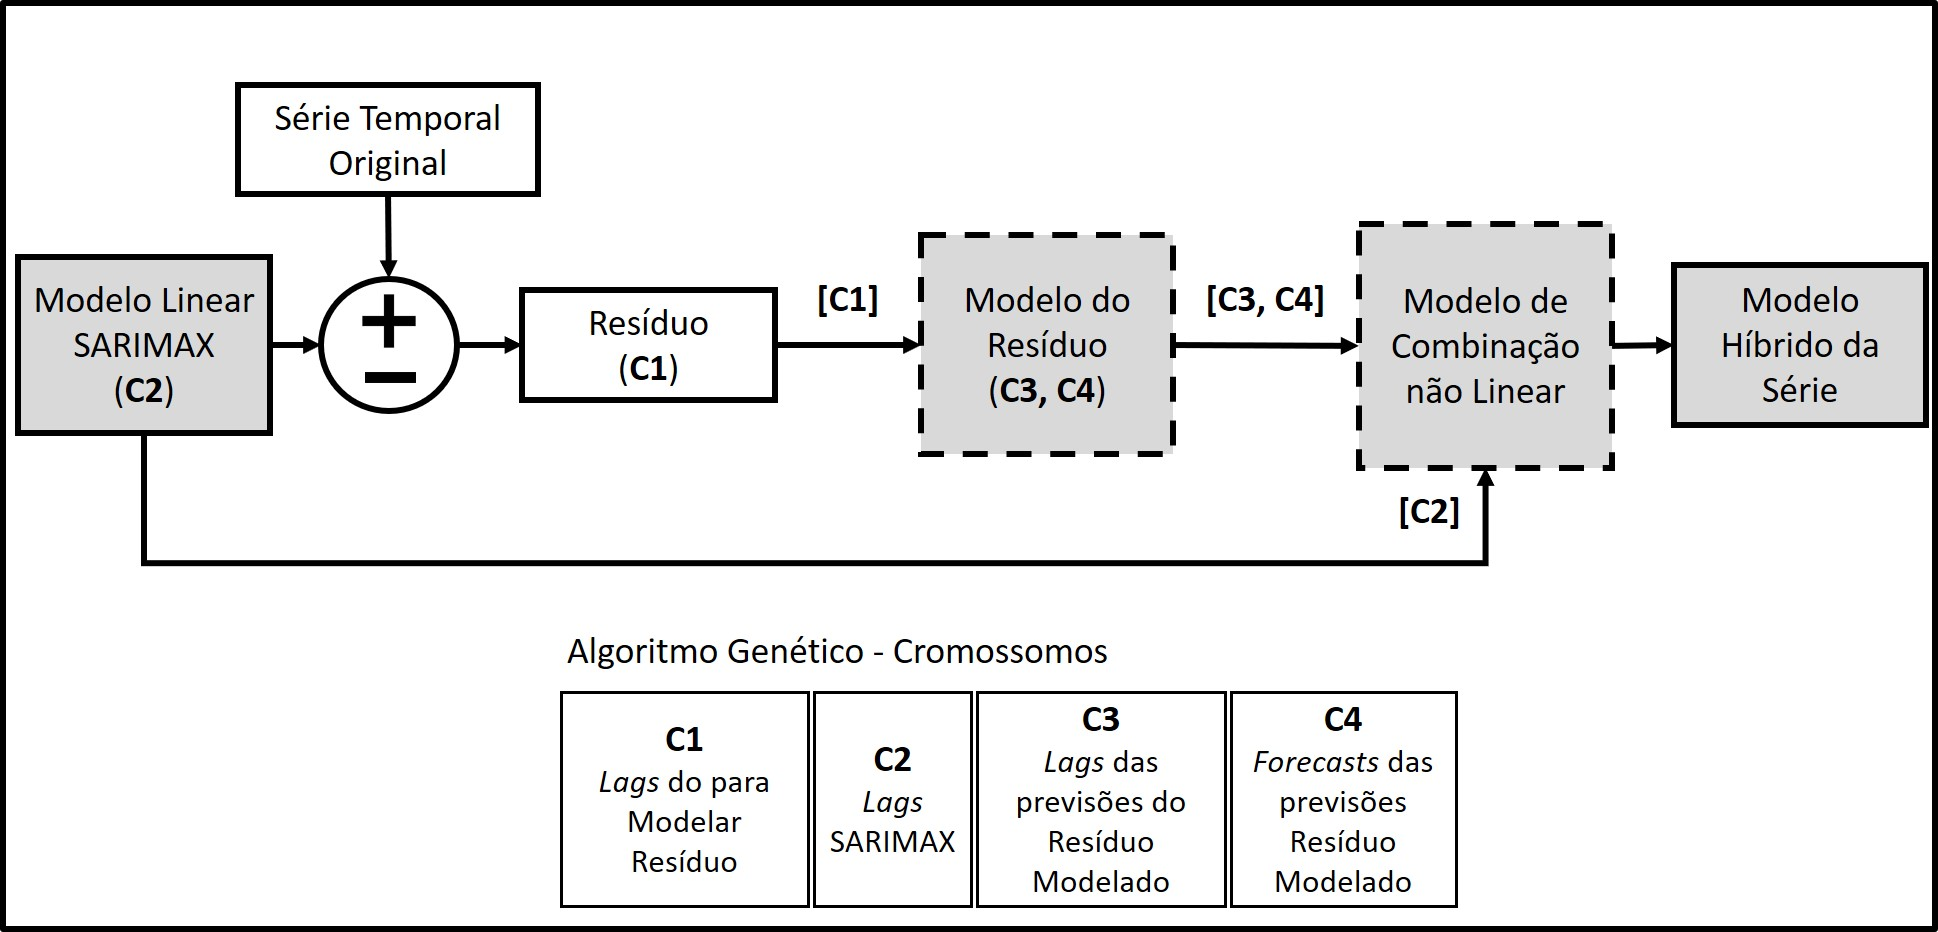
\includegraphics[width=\textwidth]{Figuras/cap5/fluxograma_cromossomos.jpg}
    \source{Autor.}
    \label{fig:cap5_fluxograma_cromossomo}
\end{figure}

Como pode ser visto, existem 4 cromossomos que são utilizados na busca por algoritmo genético. As variáveis do tipo \textit{Lags} se tratam de quantidades de amostrados do passado utilizadas para prever o futuro. Cada um dos cromossomos será melhor explicado abaixo:

\begin{itemize}
    \item C1: \textit{Lags} para Modelar Resíduo - De posse do resíduo, estas amostras são utilizadas no Modelo do Resíduo, que se trata de um objeto que também é obtido a partir de busca com algoritmo genético.
    
    \item C2: \textit{Lags} SARIMAX - De posse do Modelo Linear SARIMAX é possível obter amostras do passado da série temporal gerada por estes. Essas amostras serão utilizadas na Combinação com Amostras C3 e C4 do Resíduo Modelado.
    
    \item C3: \textit{Lags} das previsões do Resíduo Modelado - Com um Modelo ML treinado e otimizado é possível gerar a séries temporal correspondente ao Resíduo Modelado e com testa obter amostras do passado.
    
    \item C4: \textit{Forecasts} das previsões do Resíduo Modelado - Análogo ao cromossomo C3, porém com amostras a frente no tempo.
\end{itemize}

Os cromossomos C1-C4 são inicializados como números inteiros de uma distribuição uniforme de limite inferior 1 e superior 20. Foi estipulado uma probabilidade de mutação e cruzamento de 80\%.

\begin{figure}[!bp]
    \centering
    \caption{Fluxograma detalhado sobre requisitos do Modelo do Resíduo e Modelo de Combinação não Linear.}
    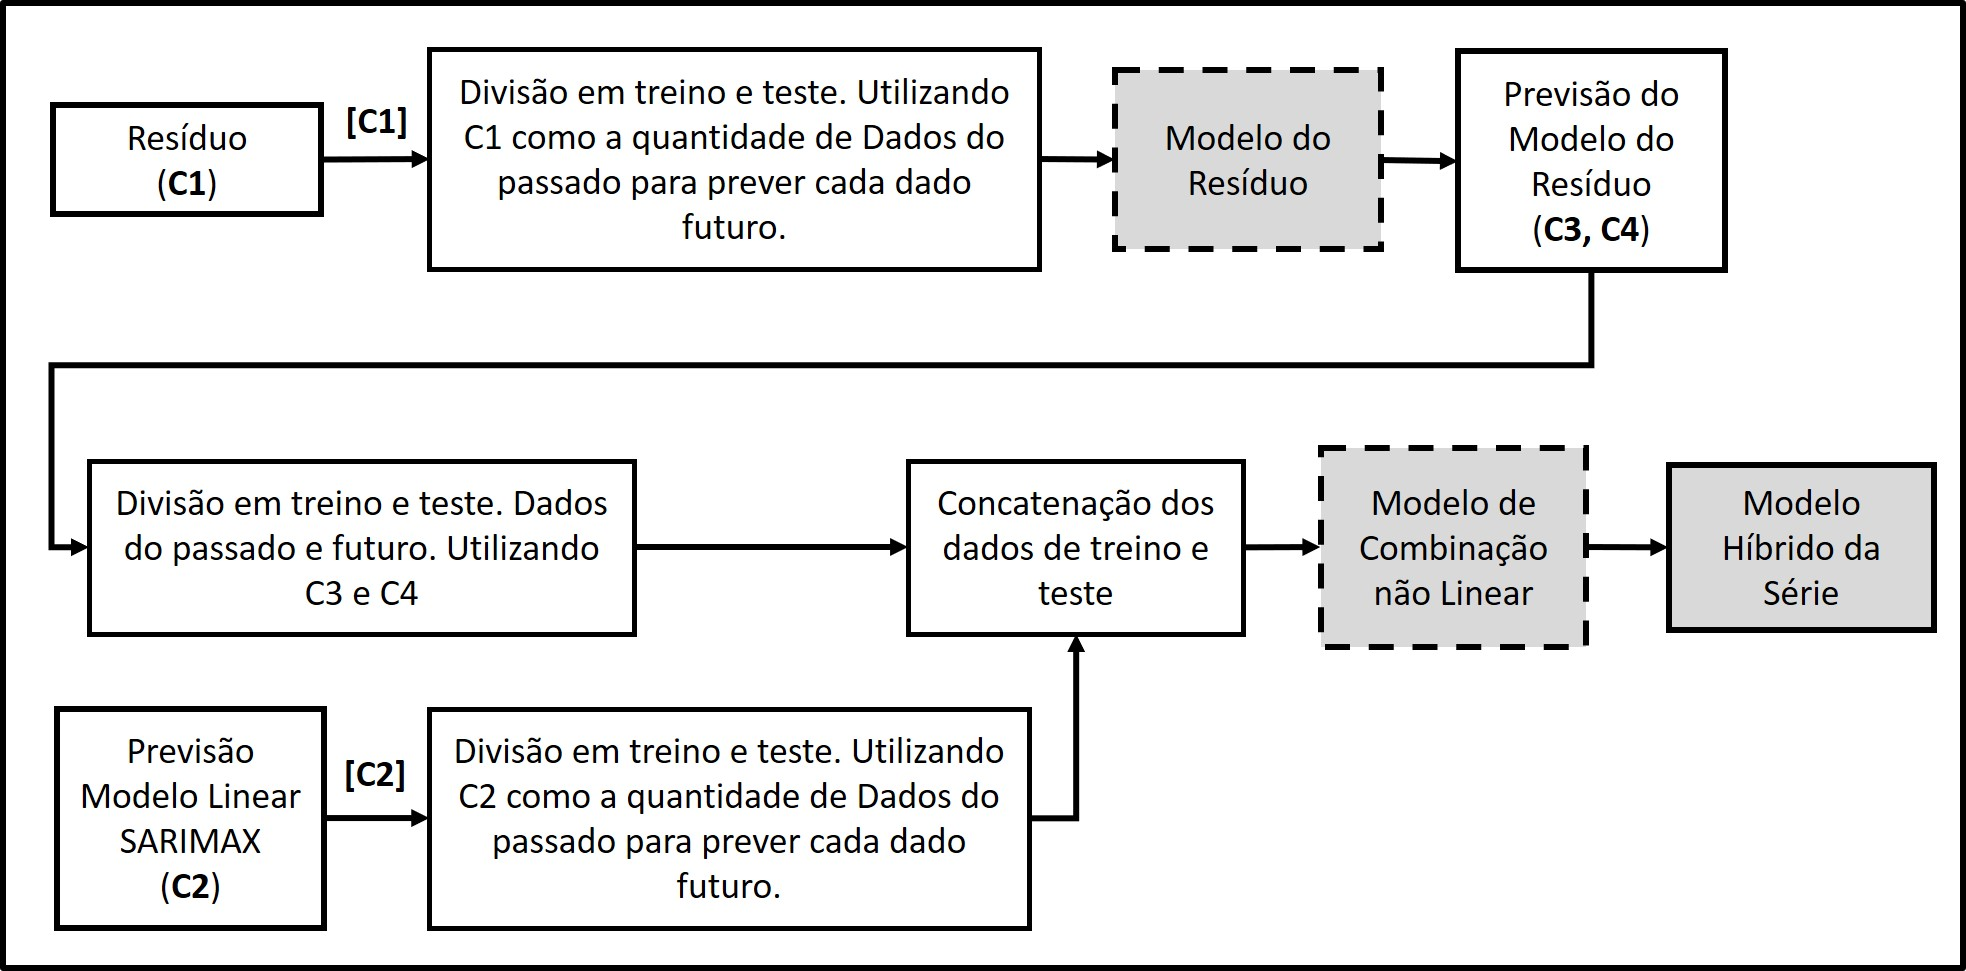
\includegraphics[width=\textwidth]{Figuras/cap5/fluxograma_modelos_res_comb.jpg}
    \source{Autor.}
    \label{fig:cap5_fluxograma_modelos_res_comb}
\end{figure}

O operador de cruzamento funciona de acordo com o Algoritmo \ref{algo:cap5_cruz_hibrid}. Os indivíduos são colocados em ordem do melhor \textit{fitness} ao pior, então o melhor indivíduo sempre é levado para a próxima população. Em seguida, para cada um dos indivíduos restantes, é definido aleatoriamente um conjunto dos quatro cromossomos que serão recebidos de um indivíduo de melhor posição, esta que é dada pela posição do individuo simetricamente. A mutação dos cromossomos se dá a partir da variação da adição de um número inteiro obtido por uma distribuição uniforme entre -2 e 2.

\begin{algorithm}[!htbp]
    \Entrada{população, Prob. Cruzamento}
    \Saida{Nova população}
    \Inicio{
    Mantém o melhor indivíduo;\\
    Ordena a população \textit{fitness} do melhor ao pior;\\
    \Para{indivíduo de ordem $I$}{
    $p$ = random(0,1);\\
    \Se{$p >$ Prob. Cruzamento}{
        $C$ = conjunto aleatório de cromossomos;\\
        população[$I$][$C$] = população[$I\slash2$][$C$]
    }
    }
    }
    \caption{Cruzamento escolhido para algoritmos híbridos propostos}
    \label{algo:cap5_cruz_hibrid}
\end{algorithm}

Ainda sobre o processo representado pela Figura \ref{fig:cap5_fluxograma_cromossomo}, é necessário explicar exatamente como as variáveis dos cromossomos são necessárias pela modelagem, esta explicação se dá melhor na Figura \ref{fig:cap5_fluxograma_modelos_res_comb}. A segunda etapa do processo é dada pelo Modelo do Resíduo e a terceira, pelo Modelo de Combinação. Em ambas estas etapas, podem ser utilizados quaisquer algoritmos de regressão para que com base nos dados de treino, se gere estes dois modelos e com dados de teste se avalie.

Neste trabalho para as etapas 2, Modelo do Resíduo e 3, Modelo de Combinação, podem ser escolhidos dois algoritmos de hiper-parametrização de MLPs, baseados em algoritmo genético, descritos nas próximas subseções \ref{subsec:ag-mlp} e \ref{subsec:ag-mlp-vr}.

\subsection{AG-MLP}
\label{subsec:ag-mlp}

Para obter a MLP bem parametrizada o algoritmo procura os melhores parâmetros para o MLP. Este tipo de otimização pode ser encontrado na literatura, sendo muito útil para aumentar a performance deste tipo de RNA \cite{ramchoun2016multilayer, idrissi2016genetic} . Nesta busca, o algoritmo gera uma população de MLPs, com parâmetros aleatórios, avalia estes e ranqueia o melhores parâmetros. Depois disso, uma nova população é gerada, após um cruzamento entre melhores e piores MLPs. A melhor MLP é repetida na próxima geração. Depois do cruzamento, os parâmetros numéricos sofrem mutação. Esta nova população é re-avaliada e o ciclo continua.

O algoritmo busca para cada MLP baseado nos cromossomos mostrados na Figura \ref{fig:cap5_cromo_mlp}. Para implementação das MLP é utilizada a biblioteca Scikit-learn do python \cite{scikit-learn}. É definido uma quantidade máxima de iterações em 500. Mais detalhadamente, cada um dos cromossomos tem as seguintes características:

\begin{figure}[bp]
    \centering
    \caption{Cromossomos do Algoritmo Genético da MLP.}
    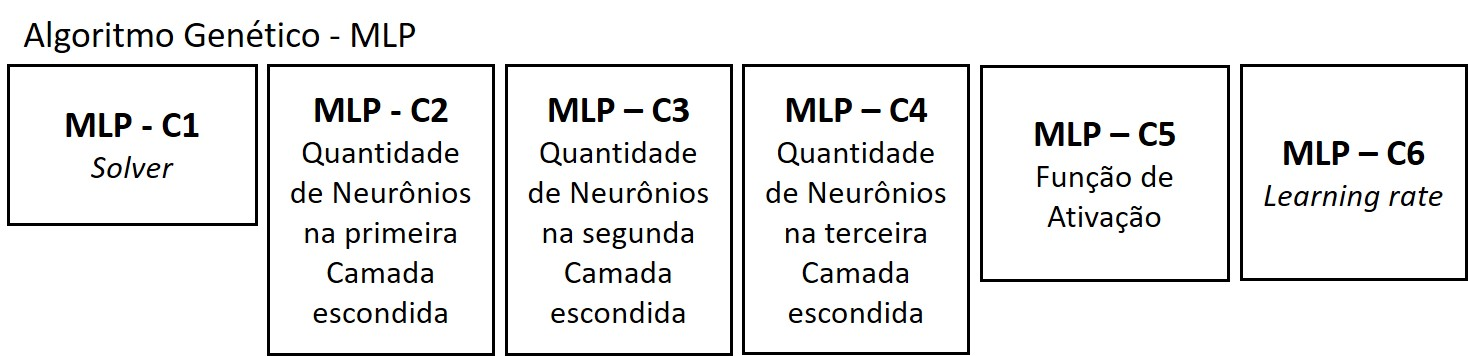
\includegraphics[width=\textwidth]{Figuras/cap5/cromo_mlp.jpg}
    \source{Autor.}
    \label{fig:cap5_cromo_mlp}
\end{figure}

\begin{itemize}
    \item MLP-C1: \textit{Solver} - Se trata do algoritmo de optimização utilizado para obter os pesos nos neurônios. Pode ser escolhido entre LBFGS, ADAM e SGD. 
    
    \item MLP-C2 à MLP-C4: Quantidade de neurônios nas camada escondida 1, 2 e 3.
    
    \item MLP-C5: Função de Ativação - Possibilidade dentre as funções Identidade, Logística, Tangente Hiperbólica e Relu.
    
    \item MLP-C6: \textit{Learning Rate} - Se trata da forma que a Taxa de Aprendizagem $\eta$ da MLP é atualizada. Pode ser escolhida entre Constante, \textit{Invscaling} e Adaptativa.
    
\end{itemize}

Sobre o cromossomo \textit{Solver}, LBFGS é um acrônimo para \textit{Limited\hyp{}Memory Broyden\hyp{}Fletcher\hyp{}Goldfarb\hyp{}Shanno Algorithm} que tende a ser mais rápido que o o algoritmo SGD, acrônimo de \textit{Stochastic Gradient Descendent} \cite{le2011optimization}. No caso de uso do SGD o momento é defidno em 0.9. ADAM, cujo nome é um derivativo de \textit{Adaptative Moment Estimation}, se trata de um algoritmo cronologicamente mais novo que os anteriores e popular em aplicações envolvendo \textit{Deep Learning} \cite{kingma2014adam, yi2020effective, jais2019adam}.

Sobre o \textit{Learning Rate}, mais detalhadamente cada uma das possibilidades é caracterizada da seguinte forma: Constante é uma taxa de aprendizagem $\eta=0,001$. \textit{Invscaling} diminui gradualmente a taxa de aprendizagem periodicamente, com período $t$ usando um expoente de escala inversa como na Equação \ref{eq:learning_rate_invscaling}. A taxa de aprendizado Adaptativa mantém a taxa de aprendizagem constante enquanto a perda de treinamento continua diminuindo. Cada vez que duas épocas consecutivas falham em diminuir a perda de treinamento em pelo menos $0,0001$, ou falham em aumentar a pontuação de validação em pelo menos $0,0001$, a taxa de aprendizado atual é dividida por 5.

\begin{equation}
\label{eq:learning_rate_invscaling}
    \begin{gathered}
    \eta = \eta \slash t^{0.5}
    \end{gathered}
\end{equation}

\subsection{AG-MLP Voting Regressor}
\label{subsec:ag-mlp-vr}

Este modelo é análogo ao da Seção \ref{subsec:ag-mlp} precedente, na utilização de MLPs como elementos principais, porém com a diferença que ao invés de se escolher uma RNA apenas para o Modelo do Resíduo e Modelo de Combinação, são escolhidas as melhores RNA de forma a ser feita uma média na predição entre as melhores. Este mecanismo é chamado de \textit{Voting Regressor}. 

Para a implementação correta deste algoritmo, é adicionado um cromossomo a mais C5 aqueles que foram explicados e ilustrados na Figura \ref{fig:cap5_fluxograma_cromossomo}. 

\begin{itemize}
    \item C5: Percentagem de MLPs que farão parte do \textit{Voting Regressor}.
\end{itemize}

O cromossomo C5 tem cruzamento equivalente ao demonstrado pelo Algoritmo \ref{algo:cap5_cruz_hibrid}, porém sua mutação dá a partir da variação da adição de um número inteiro obtido por uma distribuição uniforme entre -10 e 10. 

%\subsection{Voting Regressor Ensembles}